\documentclass{standalone}
\usepackage{tikz}
\usepackage{circuitikz}

\begin{document}
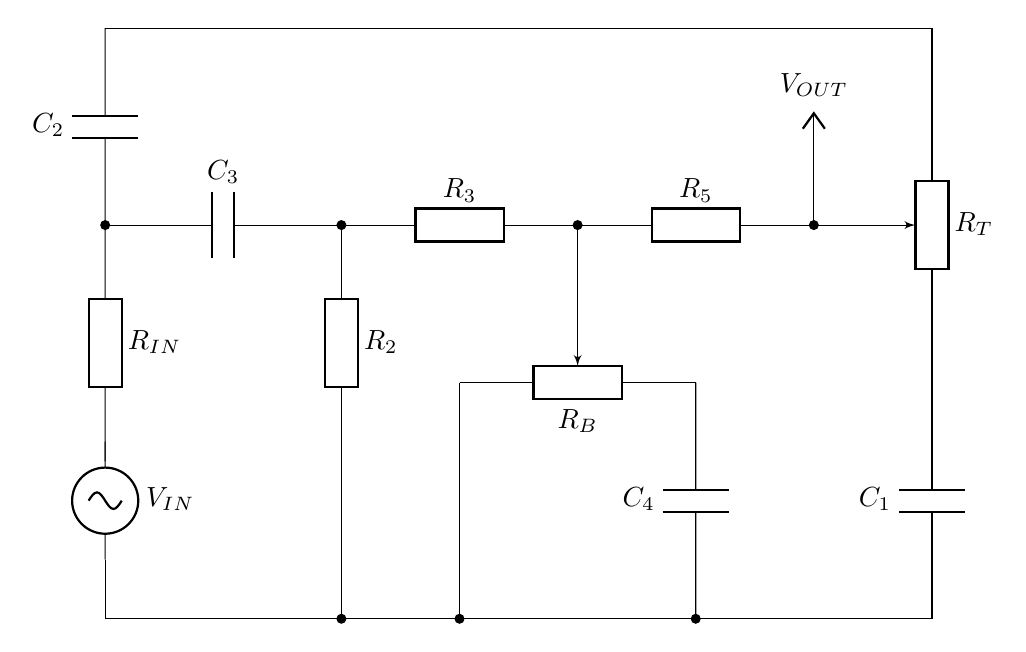
\begin{tikzpicture}
	\draw (1, 5.25) to[sinusoidal voltage source, l=$V_{IN}$] (1, 3.75);

	\draw (1, 8) to[european resistor, l=$R_{IN}$] (1, 5);
	\draw (4, 8) to[european resistor, l=$R_2$] (4, 5);
	\draw (4, 8) to[european resistor, l=$R_3$] (7, 8);
	\draw (7, 8) to[european resistor, l=$R_5$] (10, 8);

	\draw (5.5, 6) to[european potentiometer, l_=$R_B$] (8.5, 6);
	\draw (11.5, 6) to[european potentiometer, l_=$R_T$] (11.5, 10);

	\draw (11.5, 3) to[capacitor, l=$C_1$] (11.5, 6);
	\draw (1, 8) to[capacitor, l=$C_2$] (1, 10.5);
	\draw (1, 8) to[capacitor, l=$C_3$] (4, 8);
	\draw (8.5, 3) to[capacitor, l=$C_4$] (8.5, 6);

	\draw (1, 10.5) -- (11.5, 10.5) -- (11.5, 10);
	\draw (1, 3.75) -- (1, 3) -- (11.5, 3);
	\draw (4, 5) |- (4, 3);
	\draw (5.5, 6) -- (5.5, 3);
	\draw (7, 8) -- (7, 6.56);
	\draw (10.94, 8) -- (10, 8);
	\draw (10, 9) -- (10, 8);

	\node[vcc] at (10, 9) {$V_{OUT}$};
	\node[circ] at (1, 8) {};
	\node[circ] at (10, 8) {};
	\node[circ] at (4, 3) {};
	\node[circ] at (4, 8) {};
	\node[circ] at (5.5, 3) {};
	\node[circ] at (7, 8) {};
	\node[circ] at (8.5, 3) {};

\end{tikzpicture}
\end{document}